% Chapter Template

\chapter{PROPIEDADES MECANICAS DE UN BMG CON NANOPARTICULAS CRISTALINAS EMBEBIDAS} % Main chapter title

\label{C4} % Change X to a consecutive number; for referencing this chapter elsewhere, use \ref{ChapterX}

\lhead{Capítulo 4. \emph{PROPIEDADES MECANICAS DE UN BMG CON NANOPARTICULAS CRISTALINAS EMBEBIDAS}} % Change X to a consecutive number; this is for the header on each page - perhaps a shortened title

Al introucir nanopartículas a una matriz amorfa para mejorar las propiedades mecánicas (como se discute en la sección \ref{S1_3_3}) y asegurar efectos perdurables, las inclusiones deberían ser estables en el tiempo, es decir, no difundir en el material amorfo circundante perdiendo así la transición nítida entre cristal y amorfo.

En este apartado se analizan dos tipos de inclusiones cristalinas: nanopartículas de cobre cristalino con estructura de cubo centrada en las caras (Cu-FCC) y nanopartículas de cobre-circonio de fase B2 (CuZr-B2). Aunque no nos enfocamos en los efectos del tamaño de las inclusiones como otros estudios, se analiza la estabilidad de las nanopartículas a diferentes temperaturas. Durante la deformación mecánica de la muestra de un BMG con inclusiones bajo esfuerzo de tracción uniaxial, analizamos los polyedros de Voronoi y la distribución de esfuerzo y deformación cortante para estudiar el papel de la inclusión en las propiedades mecánicas de este material compuesto.

Primeramente, en la sección \ref{S4_2}, se estudia la estabilidad de la inclusión de CuZr (B2), ya que no es necesario estabilizar la fase antes de incrustar los átomos en la muestra, y esto no es posible directamente en LAMMPS. Luego, en la sección \ref{S4_3_1}, se muestran curvas de desplazamientos cuadráticos medios en función del tiempo para ambos sistemas, lo que da una idea de la estabilidad de la partícula en la matriz. Se presentan resultados tabulares de difusividad así como regresiones basadas en estos datos para mostrar la tendencia de comportamiento. En la sección \ref{S4_3_2} se presentan curvas de esfuerzo-deformación para diferentes temperaturas y ambos casos de inclusión cristalina.

Finalmente se discuten los resultados en las conclusiones, sección \ref{S4_4}

%----------------------------------------------------------------------------------------
%	SECTION 1
%----------------------------------------------------------------------------------------

\section{Detalles de la Simulación}
\label{S4_1}

Analizamos inclusiones esféricas de cobre FCC. Una región de 2 nm de radio es eliminada de la muestra en una posición central, la cual fue luego llenada con la red cristalina correspondiente, es decir, una red cristalina FCC con una constante de red de 0.3615 nm. Luego de creados los átomos de Cu en la región esférica, la configuración fue minimizada, luego equilibrada a presión cero por algunos ps, luego calentada (o enfriada) para alcanzar la temperatura final deseada (\textit{T$_{f}$}) durante 4 ps y fue finalmente recocida y templada a \textit{T$_{f}$} por 1 ns.

En esta sección nos centramos en la estabilidad de las nanopartículas a diferentes temperaturas, aunque mostraos algunos casos de sometimiento a tracción y compresión uniaxial. Una velocidad de deformación homogénea de 10$^{9}$/s es aplicada. La Difusividad en todos los casos se calcula ajustando los desplazamientos cuadráticos medios (en inglés Mean Squared Displacements o MSD), $\langle r^{2}\rangle$, obtenidos de LAMMPS.

\section{Creación de un cristal de CuZr de fase B2}
\label{S4_2}

Para incrustar estas partículas es necesario reemplazar átomos de la muestra original (estudiada en el capítulo \ref{C3}) por átomos ordenados del material buscado. LAMMPS permite el llenado directo de una región con estructura FCC, pero no así con fase B2. Es por eso que es necesario  primero crear una pequeña muestra con la estructura buscada de donde tomar el grupo de átomos necesario (en este caso, una esfera) y colocarlo en una región del mismo tamaño en la muestra original.

Creamos para esto un cubo cristalino aislado de 15 celdas unitarias de ancho para verificar el procedimiento, con una constante de celda de 3.50 \AA{}, tomado según \cite{inoue04}. Es este paso se utilizan condiciones de borde periódicas en las tres direcciones. Se realiza un proceso de minimizado de energía y relajación a presión cero. Se crean las velocidades iniciales para lograr una temperatura de 1100 K (\textit{T$_{B2}$}), según \cite{pauly10}, quien indica una temperatura de fase B2 estable entre 988 K y 1200 K. 

Se equilibra la muestra a presión cero y \textit{T$_{B2}$} en 100 ps, seguido de un recocido a \textit{T$_{B2}$} por 150 ps para ser enfriada rápidamente a 300 K a 10$^{12}$ K/s para igualar la velocidad de enfriamiento de la matriz. Los parámetros de la estructura obtenida se muestran en la Tabla \ref{C4:tb:b2CrystalParameters}.
%We first create an isolated small cubic crystal of 15 lattices wide to verify the procedure with an initial lattice constant of 3.50 \AA{}, according to \cite{inoue04}. Periodic boundaries in all directions are used in this step. This crystal is then minimized and relaxed at zero pressure. Initial velocities are created for a temperature of 1100 K (\textit{T$_{B2}$}), according to \cite{pauly10} who indicates B2 stable phase temperature between 988 K and 1200 K.
%Equilibration to zero pressure is then performed at \textit{T$_{B2}$} in 100 ps, followed by annealing at \textit{T$_{B2}$} for 150 ps and a quenching to 300 K at 10$^{12}$ K/s to match sample quenching rate. Final parameters of the created structure are shown in Table \ref{table:b2CrystalParameters}.

\begin{table}[htp]
\caption{Parámetros obtenidos para el cristal CuZr (B2)}
\begin{center}
\begin{tabular}{*{2}{c}}
\hline
Velocidad de enfriamiento [K/s] & 10$^{12}$ \\
\hline
Número de átomos & 6750 \\
\hline
Constante de celda [\AA] & 3.283 \\
\hline
Energía total (eV) & -34012.8 \\
\hline
Energía de cohesión (eV) & -5.04 \\
\hline
\end{tabular}
\end{center}
\label{C4:tb:b2CrystalParameters}
\end{table}

Luego realizamos un recocido de 100 ps a 300 K utilizando el ensamble $NVE$ de una esfera de 2 nm extraida del cristal obtenido. La Figura \ref{C4:fg:B2CuZr_Formation} \subref{C4:fg:B2Crystal} muestra el cristal resultante y la Figura \ref{C4:fg:B2CuZr_Formation} \subref{C4:fg:B2CrystalTest} muestra la evolución de la energía de cohesión en el tiempo. Es posible que la pendiente negativa en los primeros 20 ps a 25 ps sea consecuencia de una elección no óptima de la densidad inicial del cristal. Al observar que la energía se conserva en el tiempo, concluimos que la partícula así formada es estable y puede incluirse en la matriz de BMG.

%We then run a 100 ps annealing at 300 K with nve time integration of a 2 nm radius sphere cutted off the obtained cluster.
%Fgure \ref{figure:B2CuZr_Formation} \subref{figure:B2Crystal} shows the resulting crystal and figure \ref{figure:B2CuZr_Formation} \subref{figure:B2CrystalTest} shows the evolution of cohesive energy in time. The negative slope in the firsts 20-25 ps may be consequence of a not optimal initial density of the cluster. We observe that the energy is conserved and we conclude this cluster is stable to be included in the BMG sample.

\begin{figure}[htp]
\centering
\subfloat[Cristal resultante de CuZr (B2) (corte en imágen inferior)]{
	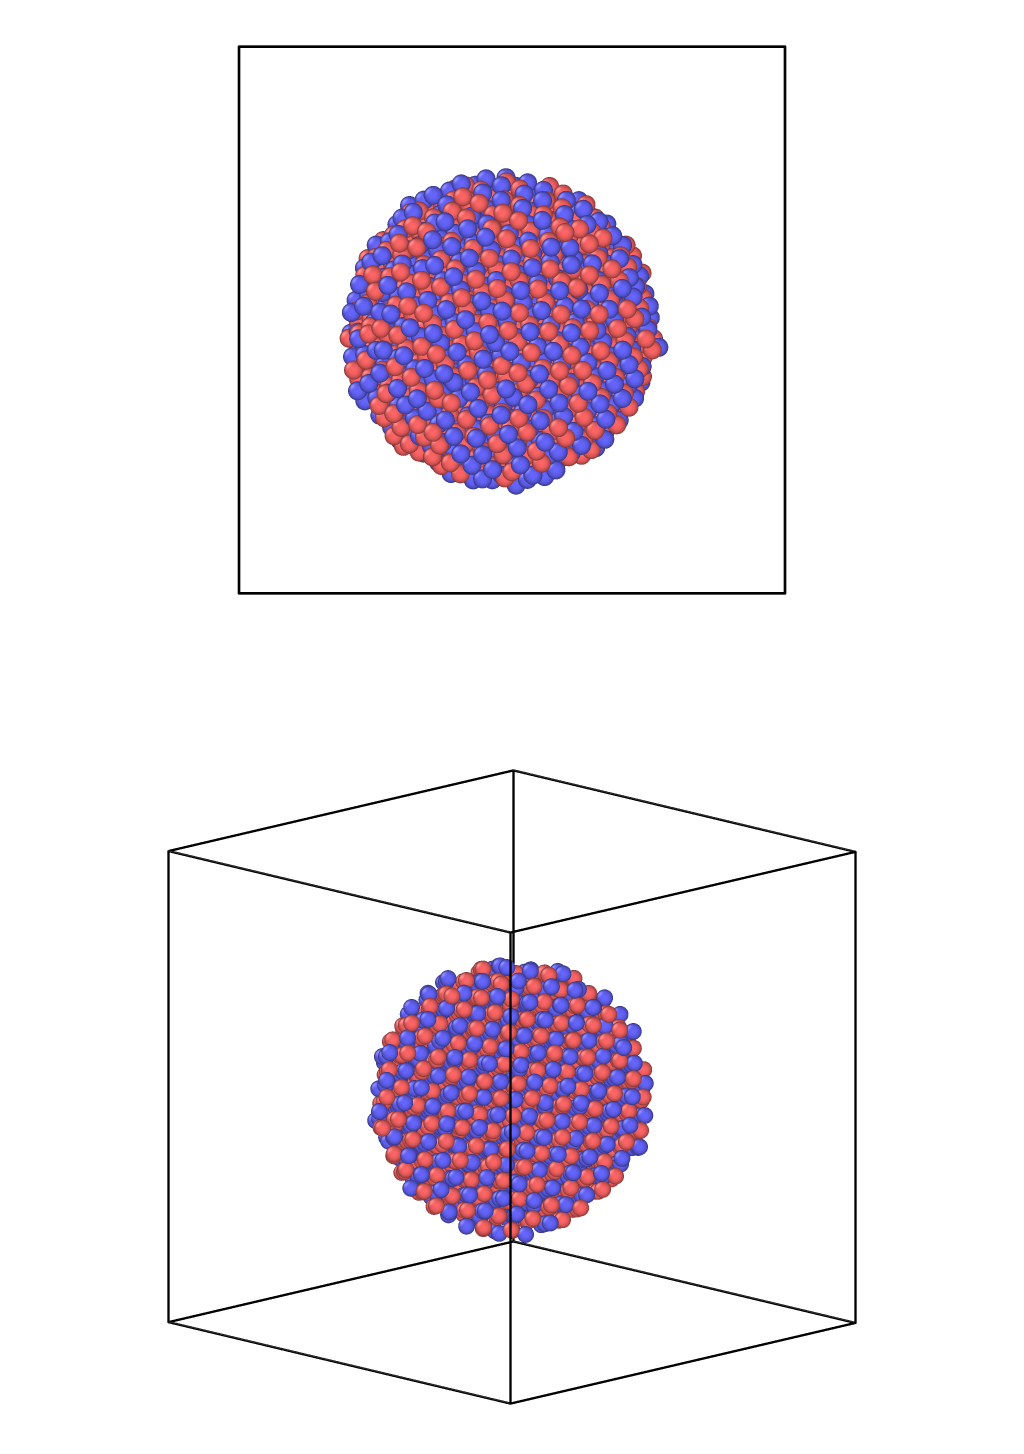
\includegraphics[width=5cm]{Cap_4/B2_FreeBoundaries.png}
	\label{C4:fg:B2Crystal}}
\quad
\subfloat[Energía de cohersión vs tiempo para el cristal de CuZr (B2) generado]{
	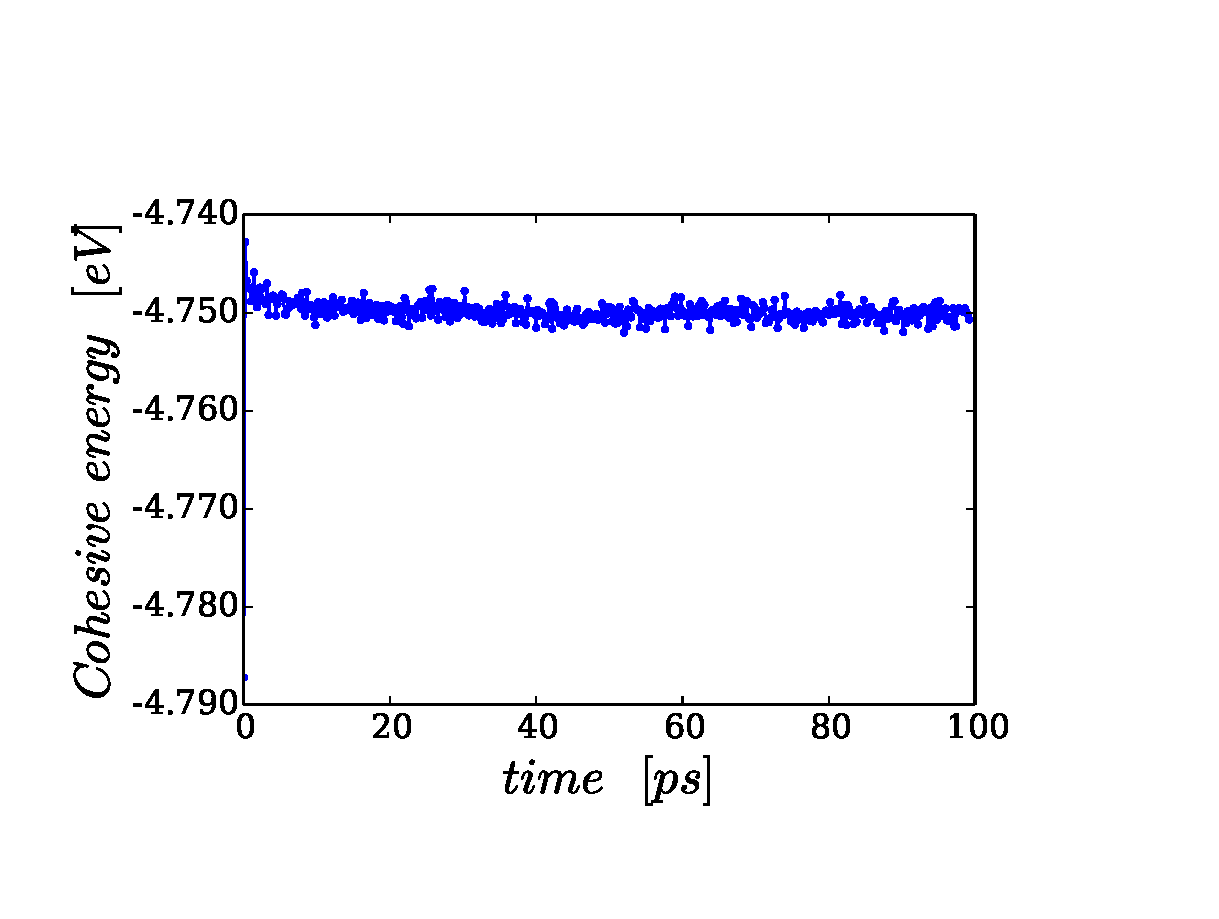
\includegraphics[width=10cm]{Cap_4/B2CrystalTest_FreeBoundariesSphere.pdf}
	\label{C4:fg:B2CrystalTest}}
\caption{Formación del cristal CuZr (B2)}
\label{C4:fg:B2CuZr_Formation}
\end{figure}

%After obtaining the initial-step configuration with this inclusion, we heat (or cool) the sample to \textit{T$_{f}$} and run an annealing for $1\,ns$, like we did with FCC-Copper inclusions.

\section{Resultados}
\label{S4_3}

En esta sección analizamos la estabilidad de nanopartículas a diferentes temperaturas, hasta temperaturas cercanas a la transición vítrea. En una primer parte, se presentan los resultados de la estabilidad de la nanopartícula y la difusividad calculada. Para tener un mismo parámetro de comparación, se utilizar los resultados obtenidos para la inclusión de Cu-FCC. Se eligen con esa información el rango de temperaturas y la ventana de tiempo tenida en cuenta. Luego se presenta la respuesta de la muesta ante esfuerzos de carga uniaxiales tanto de tracción como de compresión.

\subsection{Estabilidad de la Inclusión}
\label{S4_3_1}

La información obtenida de los MSD para los átomos de la inclusión se obtienen de simulaciones a diferentes temperaturas. Como podemos ver en la Figura \ref{C4:fg:msd_Cu_FCC} \subref{C4:fg:msd10_400_FCC}, para la nanopartícula de Cu-FCC, luego de un transitorio inicial los MSD se vuelven casi constantes, conduciendo a una difusividad cercana a cero, como es de esperar para una inclusión solida estable.

Esto indicaría que las inclusiones de Cu-FCC son de hecho estables en condiciones de operación normal para BMGs. Sin embargo, las simulaciones de MD cubren en general un corto periodo de tiempo de sólo algunos ns, y nos centramos ahora en temperaturas más elevadas para una mejor evaluación de la estabilidad de la nanopartícula. Elegimos entonces el rango de temperaturas para T $ \geq 500$ K (tanto para el caso de Cu-FCC como para el caso de CuZr-B2).

Los datos de MSD representan una media de todos los átomos de la nanopartícula, pero podrían existir grandes diferencias entre los átomos del núcleo y la superficie de la inclusión. Es por ésto que calculamos los MSD de los átomos de Cu en una región de corona esférica de un espesor de 0.8 nm y radio interno de 1.2 nm. Puede verse en la Figura \ref{C4:fg:FCCdiff_shell_comp} que, luego de un transitorio de unos 0.6 ns, las pendientes de los MSD son prácticamente iguales para la corona y la nanopartícula en su totalidad. Elegimos entonces la ventana temporal para t $ \geq 0.6 $ ns.

Las curvas de MSD para el caso de Cu-FCC se ven entonces en las Figuras \ref{C4:fg:msd_Cu_FCC} \subref{C4:fg:msd10_400_FCC} y \ref{C4:fg:msd_Cu_FCC} \subref{C4:fg:msd500_800_FCC} y para el caso de CuZr-B2 en las Figuras \ref{C4:fg:msd_CuZr_B2} \subref{C4:fg:msd10_400_B2} y \ref{C4:fg:msd_CuZr_B2} \subref{C4:fg:msd500_800_B2}.

Obtenemos entonces para T $ \geq 500$ K y t $ \geq 0.6 $ ns las difusividades que se muestran en las Tablas \ref{C4:tb:FCC_Diff_Fit_Restults} y \ref{C4:tb:B2_Diff_Fit_Restults}, usando la ecuación de Einstein $\langle r^{2}\rangle = 6Dt$.

Las difusividades son ajustadas para tener correspondencia con la ecuación \ref{C4:eq:diff_Fit}, donde $k_{B}$ es la constante de Boltzmann, $\Delta E$ es la energía de activación para difusión, y $D_{0}$ da la escala de difusividad. La regresión resultante aparece en la Tabla \ref{C4:tb:FCC_Diff_VS_T_Fit_Restults} y son mostrados gráficamente en la Figura \ref{C4:fg:FCC_diff_vs_T}. Hay que considerar que al ser tan bajos los valores obtenidos para el caso de CuZr-B2, esta regresión sólo se calcula para el caso Cu-FCC.

Es de notar que si bien las difusividades para el caso de CuZr-B2 son mucho menores (la pendiente de los movimientos atómicos es cercana a cero), el desplazamiento inicial de los átomos durante el calentamiento a la temperatura de simulación (por ejemplo desde 300 K a 500 K) es mucho mayor. En las Figuras \ref{C4:fg:heating_FCC_B2} \subref{C4:fg:heating500_800_FCC} y \ref{C4:fg:heating_FCC_B2} \subref{C4:fg:heating500_800_B2} observamos esto claramente.

Por último, como fue señalado en \cite{albe13}, el núcleo de las inclusiones se ve reducido porque los átomos más externos tienden a volverse amorfos. Este efecto se incrementa con la temperatura, como era de esperarse, cuando la difusión atómica es mayor.

\begin{figure}[htp]
\centering
\subfloat[Bajas temperaturas]{
	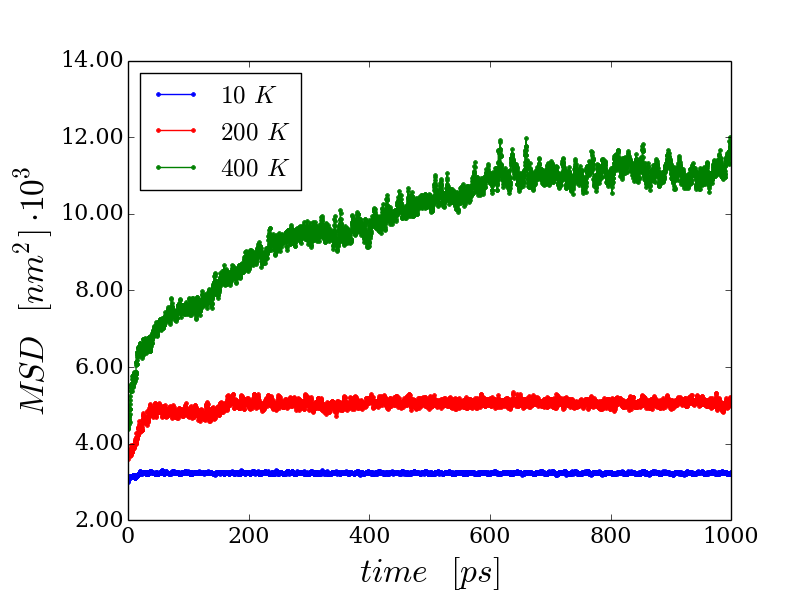
\includegraphics[width=10cm]{Cap_4/msd10_400_FCC.png}
	\label{C4:fg:msd10_400_FCC}}
\\
\subfloat[Altas temperaturas]{
	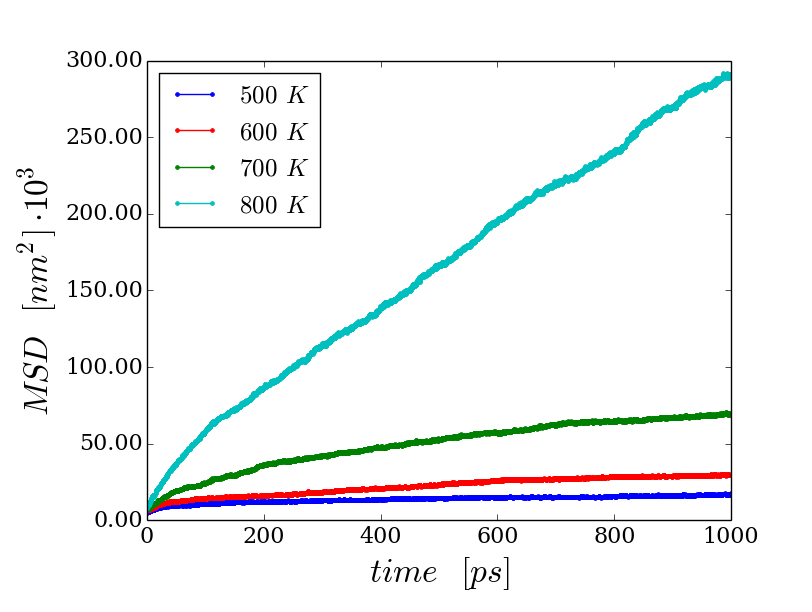
\includegraphics[width=10cm]{Cap_4/msd500_800_FCC.png}
	\label{C4:fg:msd500_800_FCC}}
\caption[MSD para inclusión de Cu FCC a diferentes temperaturas]{MSD para inclusión de Cu FCC a diferentes temperaturas}
\label{C4:fg:msd_Cu_FCC}
\end{figure}

\begin{figure}[htp]
\centering
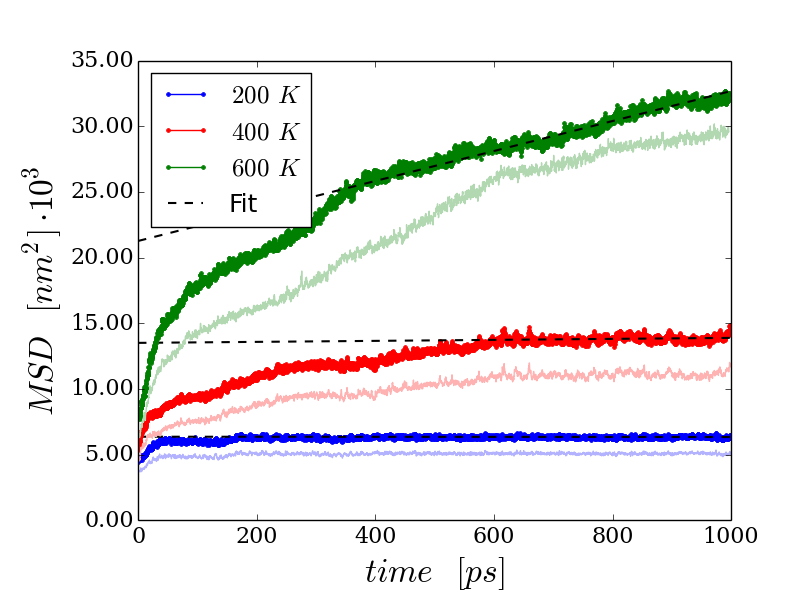
\includegraphics[width=10cm]{Cap_4/FCCdiff_shell_comp.png}
\caption[MSD de la corona esférica y la nanopartícula completa]{MSD de la corona esférica y para la nanopartícula completa (color más claro)}
\label{C4:fg:FCCdiff_shell_comp}
\end{figure}

\begin{table}[htp]
\caption{Resultados del ajuste de la difusividad para el caso Cu-FCC}
\begin{center}
\begin{tabular}{*{3}{c}}
\hline
T [$K$] & D [$\frac{nm^{2}}{ps}$] & R$^{2}$ \\
\hline \hline
500 & $8,490\cdot 10^{-7}$ & 0,8306 \\
\hline
600 & $1,508\cdot 10^{-6}$ & 0,9253 \\
\hline
700 & $4,699\cdot 10^{-6}$ & 0,9357 \\
\hline
800 & $4,149\cdot 10^{-5}$ & 0,9935 \\
\hline
\end{tabular}
\end{center}
\label{C4:tb:FCC_Diff_Fit_Restults}
\end{table}

\begin{figure}[htp]
\centering
\subfloat[Bajas temperaturas]{
	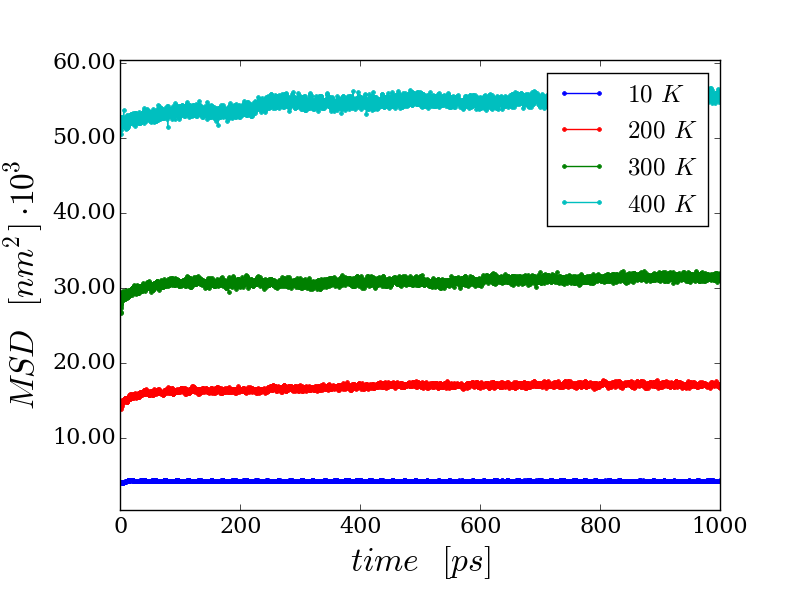
\includegraphics[width=10cm]{Cap_4/msd10_400_B2.png}
	\label{C4:fg:msd10_400_B2}}
\\
\subfloat[Altas temperaturas]{
	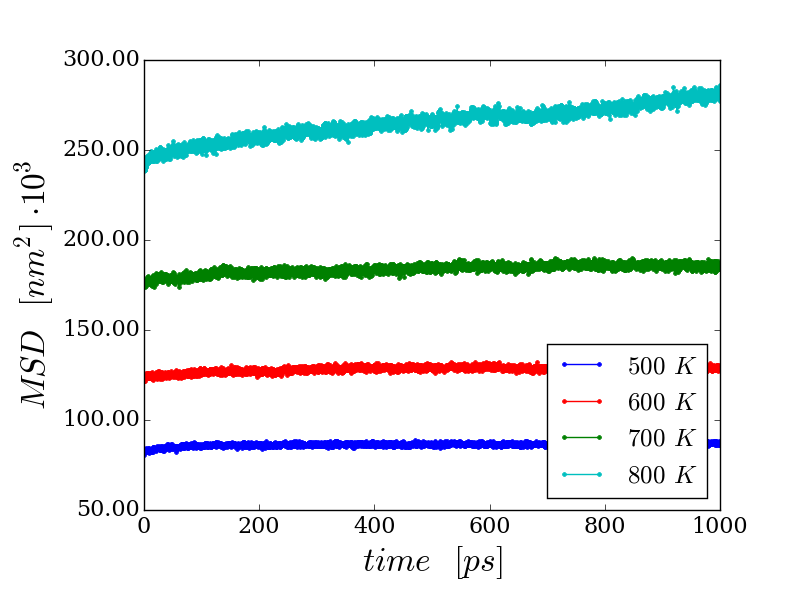
\includegraphics[width=10cm]{Cap_4/msd500_800_B2.png}
	\label{C4:fg:msd500_800_B2}}
\caption[MSD para inclusión de CuZr B2 a diferentes temperaturas]{MSD para inclusión de CuZr B2 a diferentes temperaturas}
\label{C4:fg:msd_CuZr_B2}
\end{figure}

\begin{table}[htp]
\caption{Resultados del ajuste de la difusividad para el caso CuZr-B2}
\begin{center}
\begin{tabular}{*{3}{c}}
\hline
T [$K$] & D [$\frac{nm^{2}}{ps}$] & R$^{2}$ \\
\hline \hline
500 & $2,104\cdot 10^{-7}$ & 0,0452 \\
\hline
600 & $7,094\cdot 10^{-8}$ & 0,0026 \\
\hline
700 & $2,122\cdot 10^{-7}$ & 0,0112 \\
\hline
800 & $5,712\cdot 10^{-6}$ & 0,7940 \\
\hline
\end{tabular}
\end{center}
\label{C4:tb:B2_Diff_Fit_Restults}
\end{table}

\begin{eqnarray}
D = D_{0}\cdot \mathrm{e}^{\frac{-\Delta E}{k_{B} T}}
\label{C4:eq:diff_Fit}
\end{eqnarray}

\begin{figure}[htp]
\centering
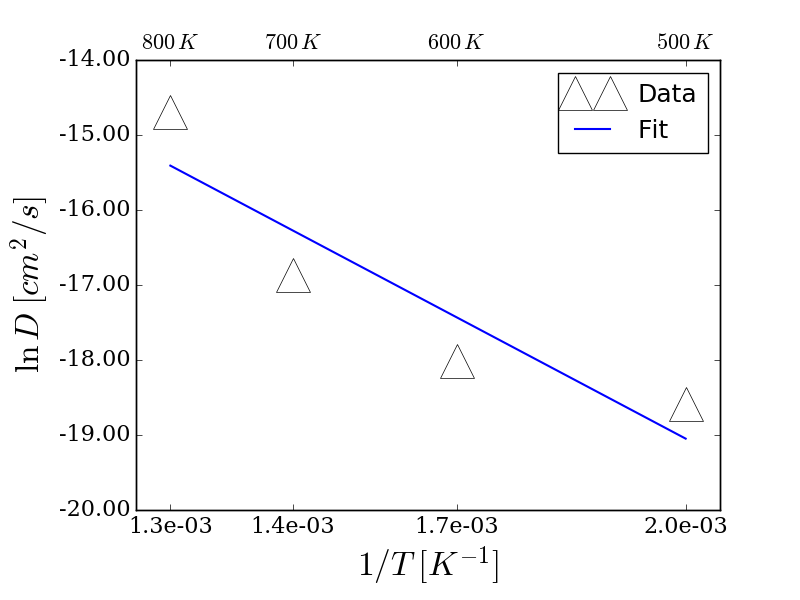
\includegraphics[width=10cm]{Cap_4/FCCDiff_vs_temp_fit.png}
\caption[Difusividad en función de la temperatura (Cu-FCC)]{Difusividad en función de la temperatura para el caso Cu-FCC}
\label{C4:fg:FCC_diff_vs_T}
\end{figure}

\begin{table}[htp]
\caption{Resultados del ajuste de la difusividad con respecto a la temperatura (inclusión de Cu-FCC)}
\begin{center}
\begin{tabular}{*{2}{c}}
\hline
Energía de activación [$eV$]& $-0,4182$ \\
\hline \hline
D$_{0}$ [$\frac{nm^{2}}{ps}$] & $8,771\times 10^{-3}$\\
\hline
R$^{2}$ & 0.8399 \\
\hline
\end{tabular}
\end{center}
\label{C4:tb:FCC_Diff_VS_T_Fit_Restults}
\end{table}

\begin{figure}[htp]
\centering
\subfloat[Nanopartícula Cu-FCC]{
	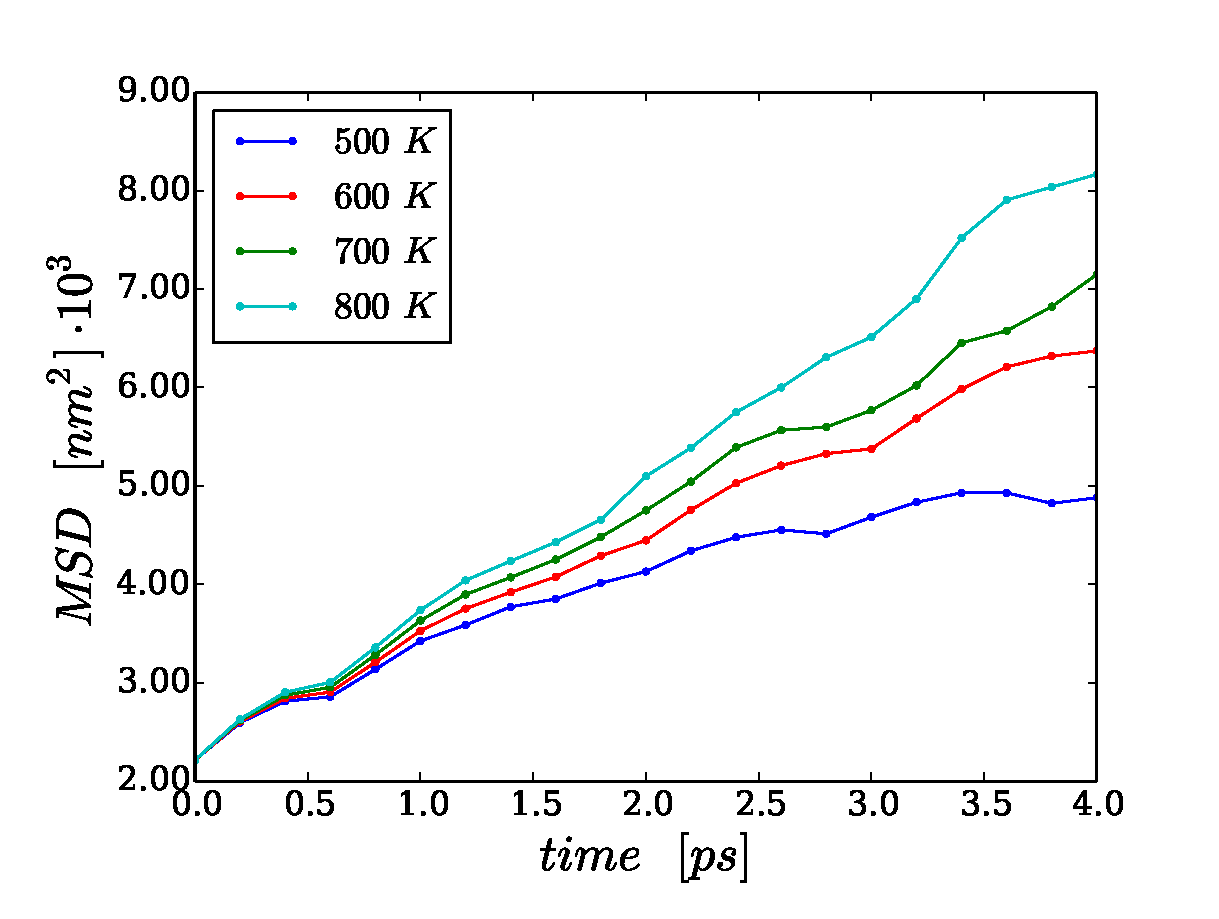
\includegraphics[width=10cm]{Cap_4/heatingFCC_500_800.pdf}
	\label{C4:fg:heating500_800_FCC}}
\\
\subfloat[Nanopartícula CuZr-B2]{
	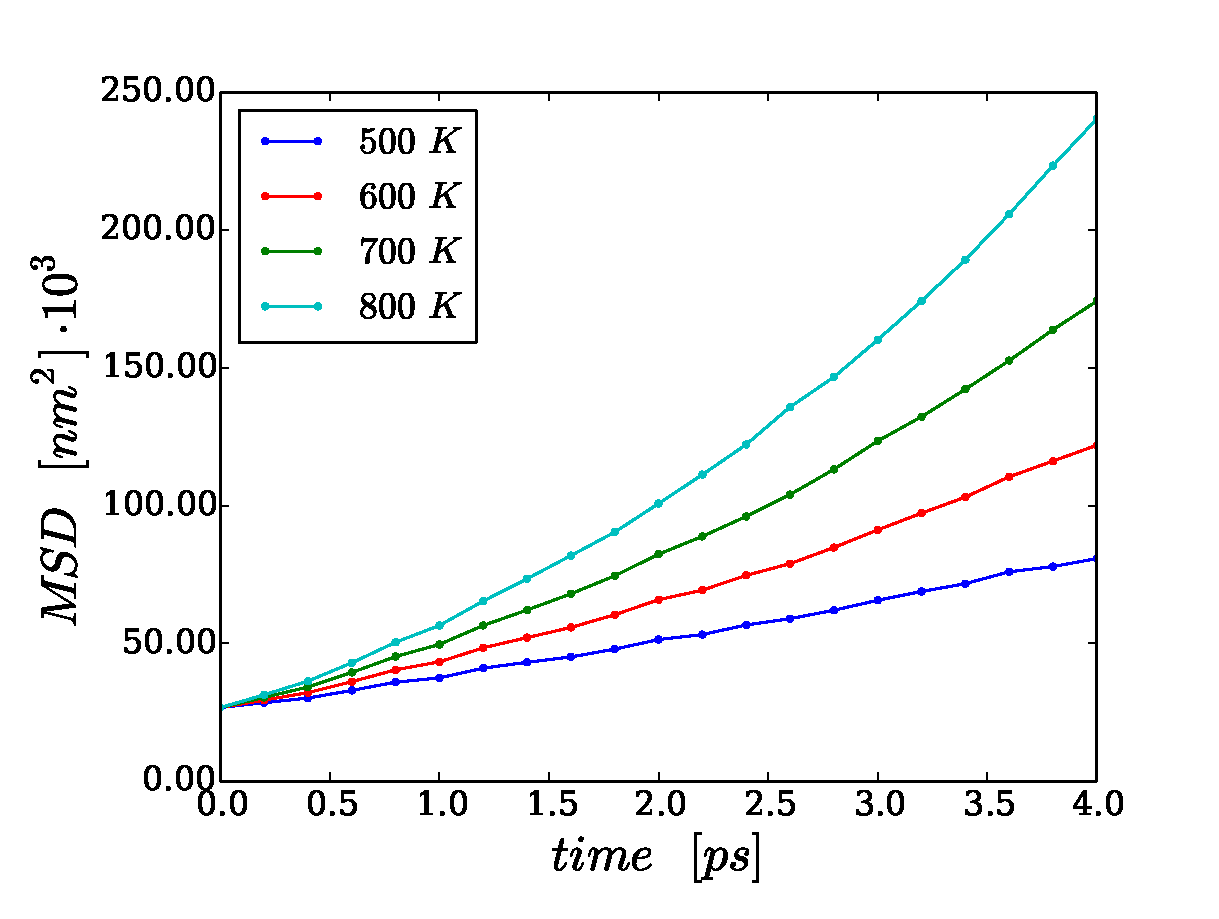
\includegraphics[width=10cm]{Cap_4/heatingB2_500_800.pdf}
	\label{C4:fg:heating500_800_B2}}
\caption[MSD para t $ \leq 4 $ ns. Ambas nanopartículas]{MSD para t $ \leq 4 $ ns. Ambas nanopartículas}
\label{C4:fg:heating_FCC_B2}
\end{figure}

\subsection{Carga Uniaxial del BMG}
\label{S4_3_2}

En esta sección, presentamos resultados sobre el sometimiento a esfuerzos uniaxiales del BMG que contiene una nanopartícula, como se describió anteriormente.

Las Figuras \ref{C4:fg:fcc_vm_tension} a \ref{C4:fg:b2_vm_compression} muestran el comportamiento esfuerzo-deformación de la muestra bajo esfuerzos uniaxiales de tracción y compresión a diferentes temperaturas. La apariencia de estas curvas sigue un comportamiento esperado observado para el material sin ninguna inclusión. La pequeña inclusión no afecta el régimen elástico, y a una temperatura elevada, el ablandamiento del BMG tampoco es afectado, tanto para tracción como para compresión. El esfuerzo máximo se ve decrementado ligeramente por la nanopartícula a bajas temperaturas. El esfuerzo de FLUJO PLASTICO(?) a grandes deformaciones no se ve modificado por la inclusión bajo compresión.

Si bien sería de esperar que los esfuerzos se concentren en la frontera entre la inclusión cristalina y la matriz amorfa, como vemos en las Figuras \ref{C4:fg:snapshot_ten_FCC_10K} a \ref{C4:fg:snapshot_comp_B2_400K} en general encontramos deformación plástica homogénea con nucleación abundante de STZs, probablemente debido a la alta velocidad de deformación y alta velocidad de templado de la muestra. Para el caso de esfuerzos de tracción (Figuras \ref{C4:fg:snapshot_ten_FCC_10K} a \ref{C4:fg:snapshot_ten_FCC_400K} y \ref{C4:fg:snapshot_ten_B2_10K} a \ref{C4:fg:snapshot_ten_B2_400K}) existe uno o más poros nucleados llegada una determinada deformación. El momento de su apertura coincide con la caída en el esfuerzo que observamos claramente en las Figuras \ref{C4:fg:fcc_vm_tension} y \ref{C4:fg:b2_vm_tension}. Para el caso de esfuerzos de compresión se observa un comportamiento similar en cuanto a la distribución homogénea de esfuerzos en la matriz amorfa.

La nucleación de los poros bajo tracción se ve algo retrasada por la inclusión, permitiendo alrededor de un 1\% de deformación adicional de la muestra en el caso general. Ésto podría explicarse por alguna relajación y disipación ocurriendo en la frontera entre la nanopartícula y el BMG, pero un estudio más detallado debería realizarse para aclarar la situación ya que en el caso particular de la inclusión CuZr-B2 a 200 K observamos una caída anticipada del esfuerzo.

Como algunos poliedros de Voronoi son considerados ser estructuras más resistentes al esfuerzo cortante, particularmente las agrupaciones de icosaedros \cite{cheng08}, mostramos la evolución de la fracción de icosaedros en la muestra y la comparamos con la muestra de BMG original sin inclusiones y a 10 K. Podemos ver en la figura \ref{C4:fg:fcc_voro_10K} que las fracciones siguen el mismo comportamiento que en la muestra sin nanopartícula. Bajo tracción, la nucleación de un poro da origen a fluctuaciones. Vale la pena notar que estas fluctuaciones corresponden a una deformación más elevada como ya se había mencionado para la curva de esfuerzo-deformación.

\begin{figure}[htp]
\centering
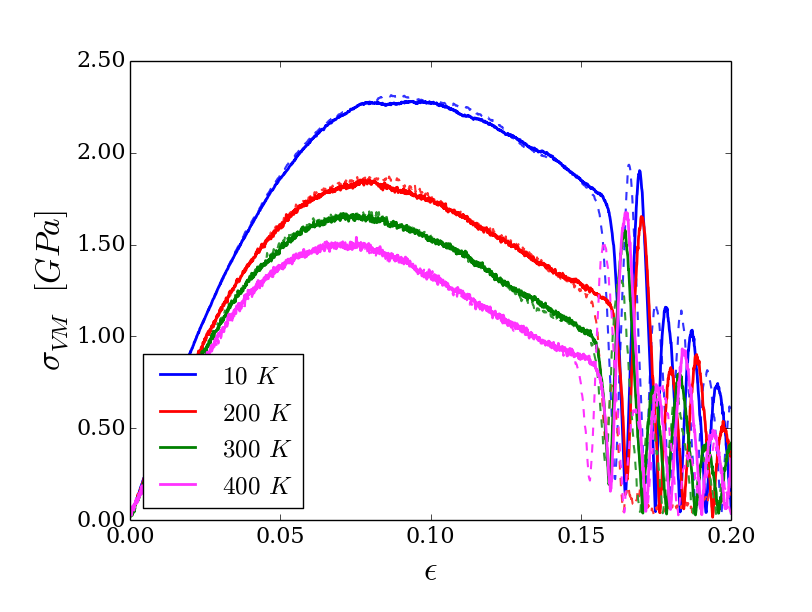
\includegraphics[width=10cm]{Cap_4/stress_strain_tension_FCC_NoInc.png}
\caption[vonMises vs deformación en tracción. Inclusión Cu-FCC]{Tensión de vonMises vs deformación para el BMG bajo esfuerzo uniaxial de tracción sin inclusión (línea punteada) y una inclusión de Cu-FCC (línea sólida)}
\label{C4:fg:fcc_vm_tension}
\end{figure}

\begin{figure}[htp]
\centering
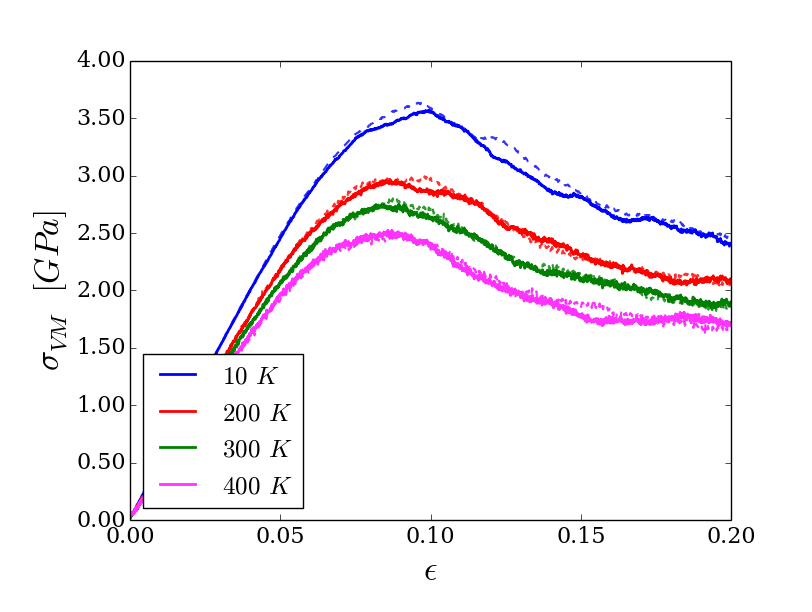
\includegraphics[width=10cm]{Cap_4/stress_strain_compression_FCC_NoInc.png}
\caption[vonMises vs deformación en compresión. Inclusión de Cu-FCC]{Tensión de vonMises vs deformación para el BMG bajo esfuerzo uniaxial de compresión sin inclusión (línea punteada) y una inclusión de Cu-FCC (línea sólida)}
\label{C4:fg:fcc_vm_compression}
\end{figure}

\begin{figure}[htp]
\centering
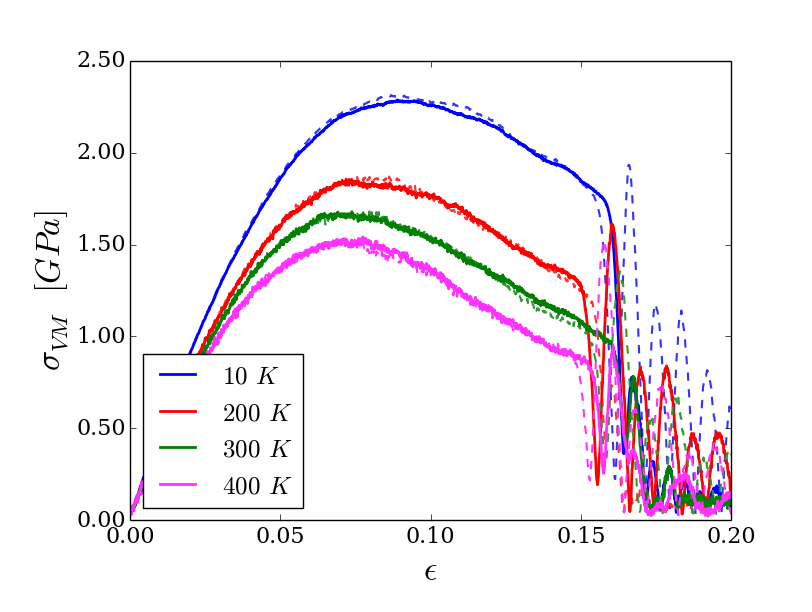
\includegraphics[width=10cm]{Cap_4/stress_strain_tension_B2_NoInc.png}
\caption[vonMises vs deformación en tracción. Inclusión de CuZr-B2]{Tensión de vonMises vs deformación para el BMG bajo esfuerzo uniaxial de tracción sin inclusión (línea punteada) y una inclusión de CuZr-B2 (línea sólida)}
\label{C4:fg:b2_vm_tension}
\end{figure}

\begin{figure}[htp]
\centering
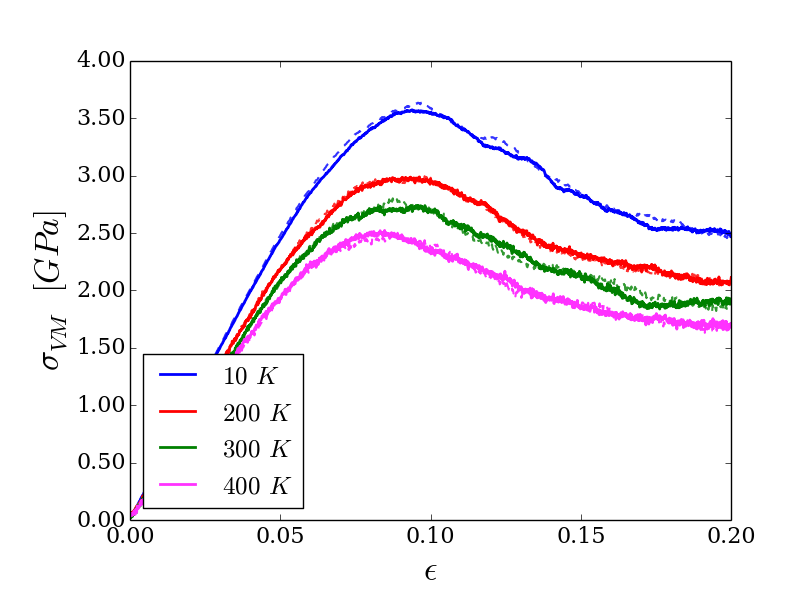
\includegraphics[width=10cm]{Cap_4/stress_strain_compression_B2_NoInc.png}
\caption[vonMises vs deformación en compresión. Inclusión de CuZr-B2]{Tensión de vonMises vs deformación para el BMG bajo esfuerzo uniaxial de compresión sin inclusión (línea punteada) y una inclusión de CuZr-B2 (línea sólida)}
\label{C4:fg:b2_vm_compression}
\end{figure}

\begin{figure}[htp]
\centering
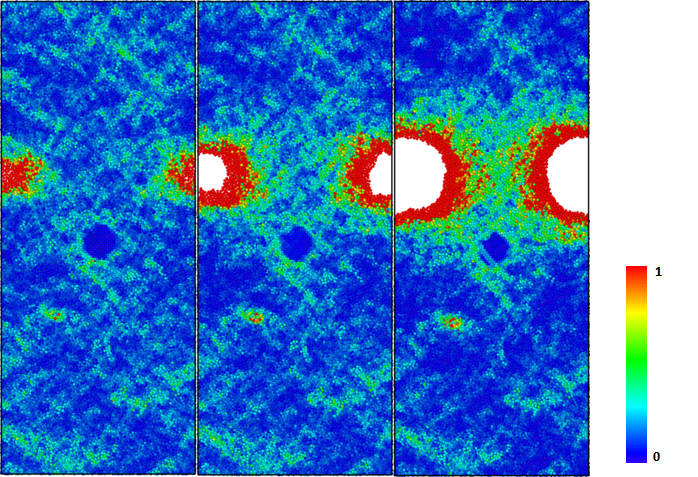
\includegraphics[width=10cm]{../ResumenImagenes/Figures/NanoParticles/Snapshots/cuSphereTension_10K_Snapshots.png}
\caption{Inclusión de Cu-FCC bajo tracción a 10K}
\label{C4:fg:snapshot_ten_FCC_10K}
\end{figure}

% \begin{figure}[htp]
% \centering
% 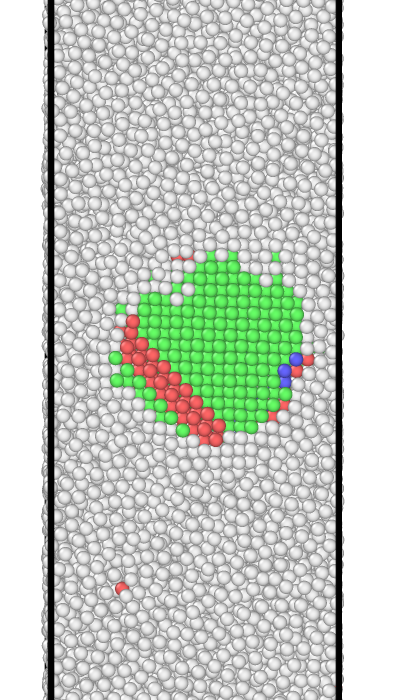
\includegraphics[width=10cm]{../ResumenImagenes/Figures/NanoParticles/cuSphereTension_10K_Snapshot_670_Macla_A.png}
% \caption{Dislocación al traccionar la muestra con nanopartícula de Cu-FCC a 10K (A). Verde: FCC, Rojo: HCP}
% \label{C4:fg:dislocacion_A}
% \end{figure}
% 
% \begin{figure}[htp]
% \centering
% 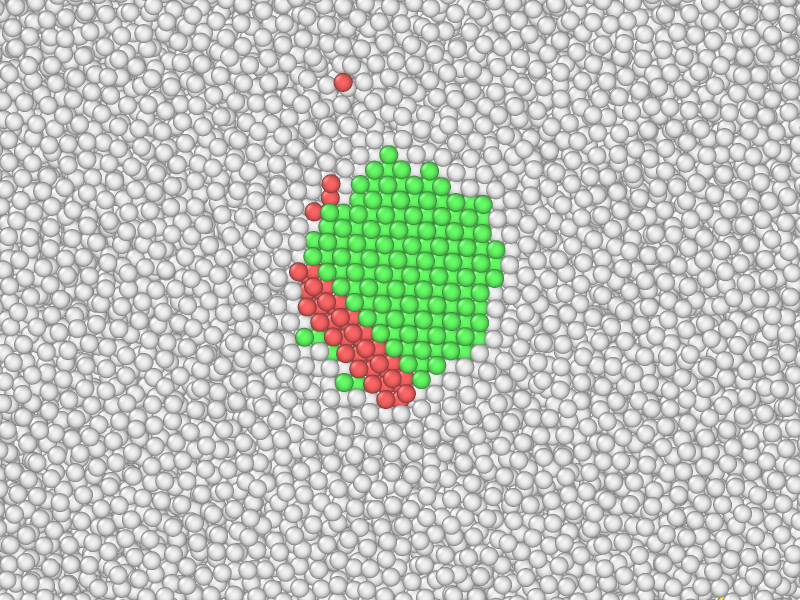
\includegraphics[width=10cm]{../ResumenImagenes/Figures/NanoParticles/cuSphereTension_10K_Snapshot_670_Macla_B.png}
% \caption{Dislocación al traccionar la muestra con nanopartícula de Cu-FCC a 10K (B). Verde: FCC, Rojo: HCP}
% \label{C4:fg:dislocacion_B}
% \end{figure}

\begin{figure}[htp]
\centering
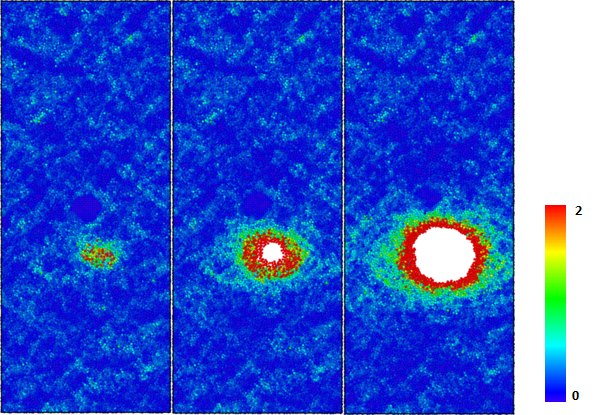
\includegraphics[width=10cm]{../ResumenImagenes/Figures/NanoParticles/Snapshots/cuSphereTension_200K_Snapshots.png}
\caption{Inclusión de Cu-FCC bajo tracción a 200K}
\label{C4:fg:snapshot_ten_FCC_200K}
\end{figure}

\begin{figure}[htp]
\centering
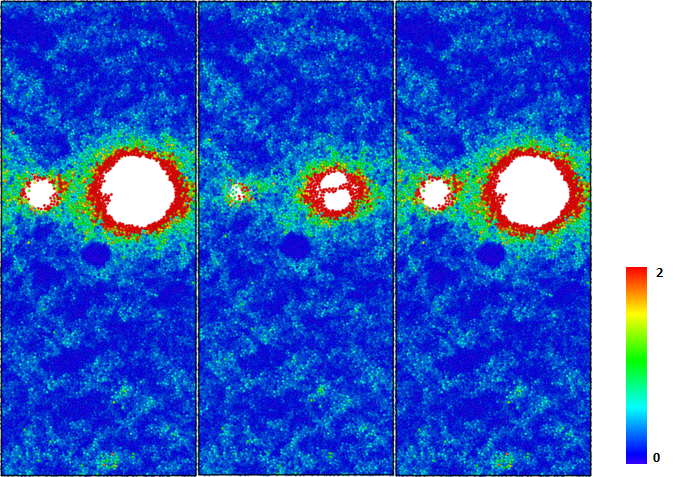
\includegraphics[width=10cm]{../ResumenImagenes/Figures/NanoParticles/Snapshots/cuSphereTension_400K_Snapshots.png}
\caption{Inclusión de Cu-FCC bajo tracción a 400K}
\label{C4:fg:snapshot_ten_FCC_400K}
\end{figure}

\begin{figure}[htp]
\centering
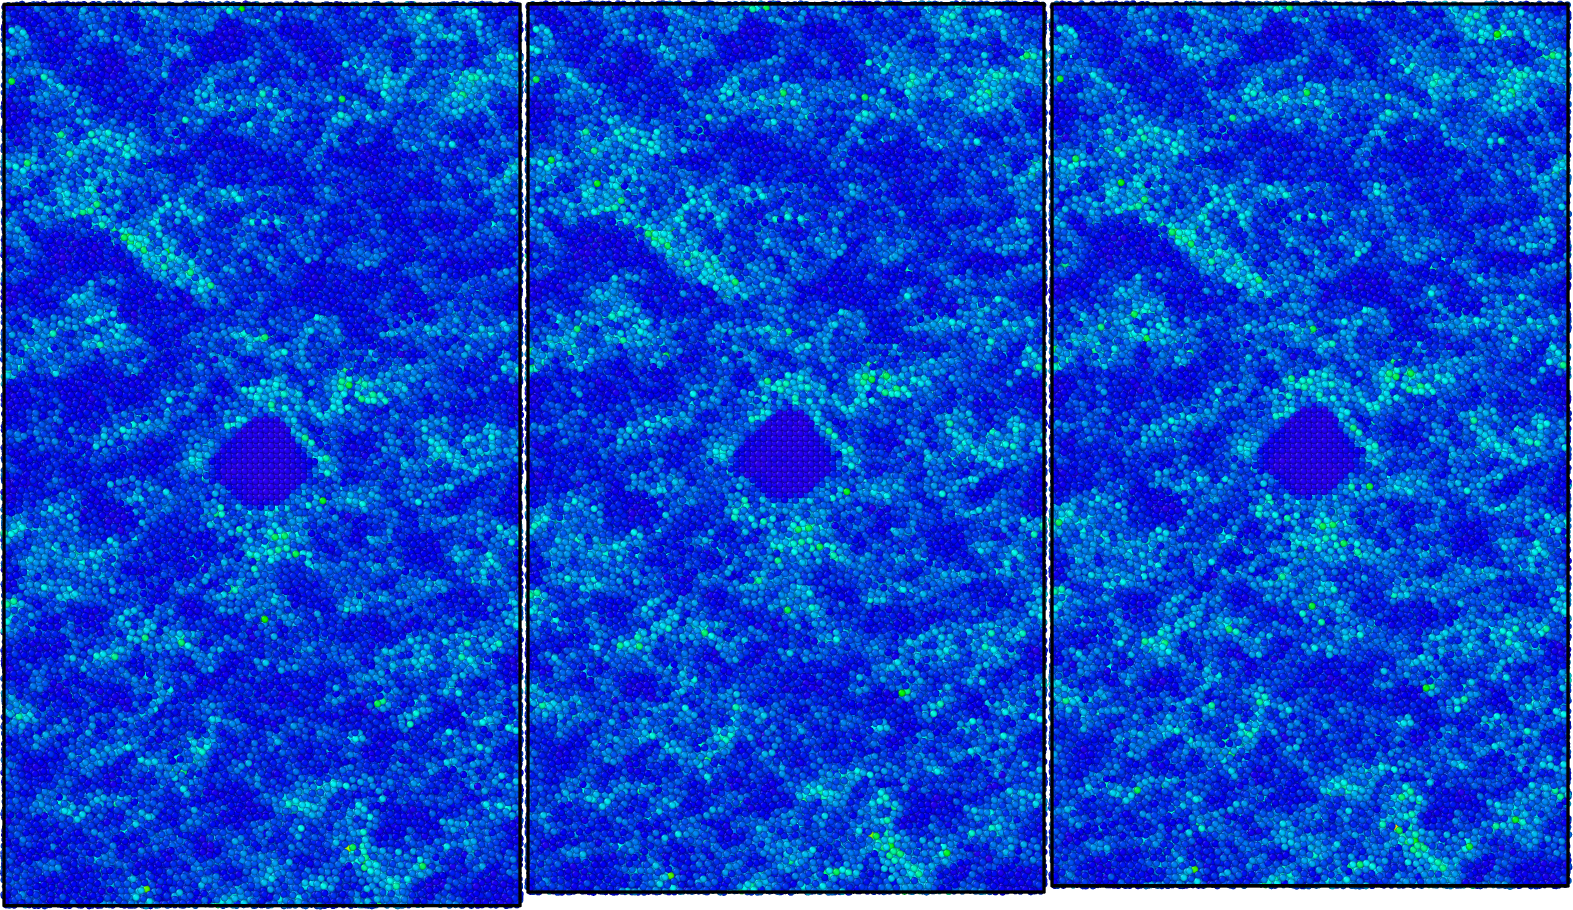
\includegraphics[width=10cm]{../ResumenImagenes/Figures/NanoParticles/Snapshots/cuSphereCompression_10K_Snapshots.png}
\caption{Inclusión de Cu-FCC bajo compresión a 10K}
\label{C4:fg:snapshot_comp_FCC_10K}
\end{figure}

\begin{figure}[htp]
\centering
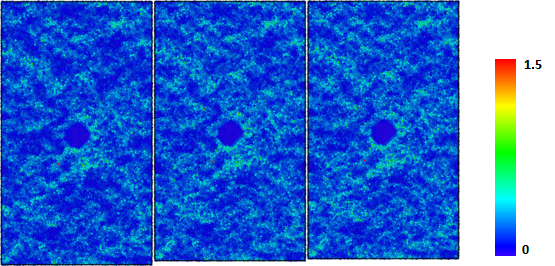
\includegraphics[width=10cm]{../ResumenImagenes/Figures/NanoParticles/Snapshots/cuSphereCompression_200K_Snapshots.png}
\caption{Inclusión de Cu-FCC bajo compresión a 200K}
\label{C4:fg:snapshot_comp_FCC_200K}
\end{figure}

\begin{figure}[htp]
\centering
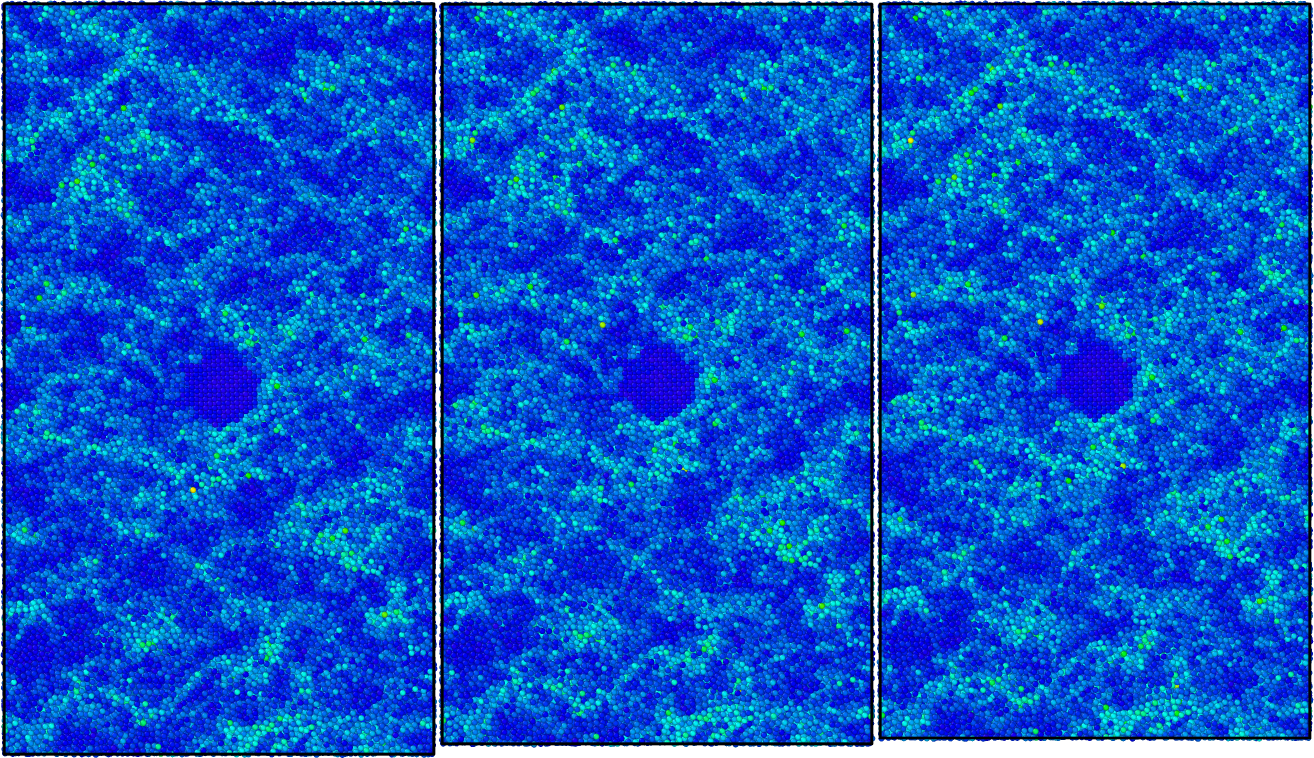
\includegraphics[width=10cm]{../ResumenImagenes/Figures/NanoParticles/Snapshots/cuSphereCompression_300K_Snapshots.png}
\caption{Inclusión de Cu-FCC bajo compresión a 300K}
\label{C4:fg:snapshot_comp_FCC_300K}
\end{figure}

\begin{figure}[htp]
\centering
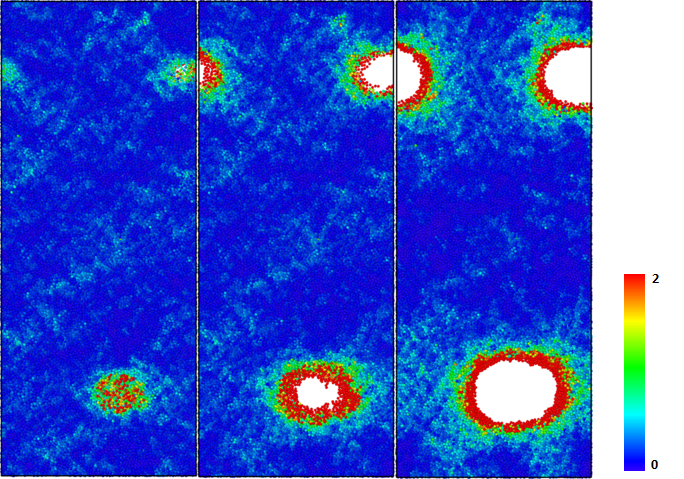
\includegraphics[width=10cm]{../ResumenImagenes/Figures/NanoParticles/Snapshots/B2SphereTension_10K_Snapshots.png}
\caption{Inclusión de CuZr-B2 bajo tracción a 10K}
\label{C4:fg:snapshot_ten_B2_10K}
\end{figure}

\begin{figure}[htp]
\centering
\includegraphics[width=10cm]{../ResumenImagenes/Figures/NanoParticles/Snapshots/B2SphereTension_200K_Snapshots.png}
\caption{Inclusión de CuZr-B2 bajo tracción a 200K}
\label{C4:fg:snapshot_ten_B2_200K}
\end{figure}

\begin{figure}[htp]
\centering
\includegraphics[width=10cm]{../ResumenImagenes/Figures/NanoParticles/Snapshots/B2SphereTension_300K_Snapshots.png}
\caption{Inclusión de CuZr-B2 bajo tracción a 300K}
\label{C4:fg:snapshot_ten_B2_300K}
\end{figure}

\clearpage

\begin{figure}[htp]
\centering
\includegraphics[width=10cm]{../ResumenImagenes/Figures/NanoParticles/Snapshots/B2SphereTension_400K_Snapshots.png}
\caption{Inclusión de CuZr-B2 bajo tracción a 400K}
\label{C4:fg:snapshot_ten_B2_400K}
\end{figure}

\begin{figure}[htp]
\centering
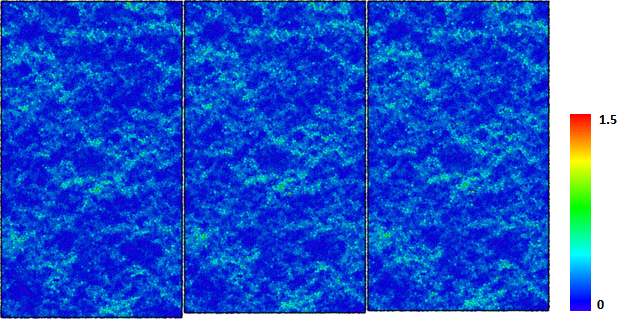
\includegraphics[width=10cm]{../ResumenImagenes/Figures/NanoParticles/Snapshots/B2SphereCompression_10K_Snapshots.png}
\caption{Inclusión de CuZr-B2 bajo compresión a 10K}
\label{C4:fg:snapshot_comp_B2_10K}
\end{figure}

\begin{figure}[htp]
\centering
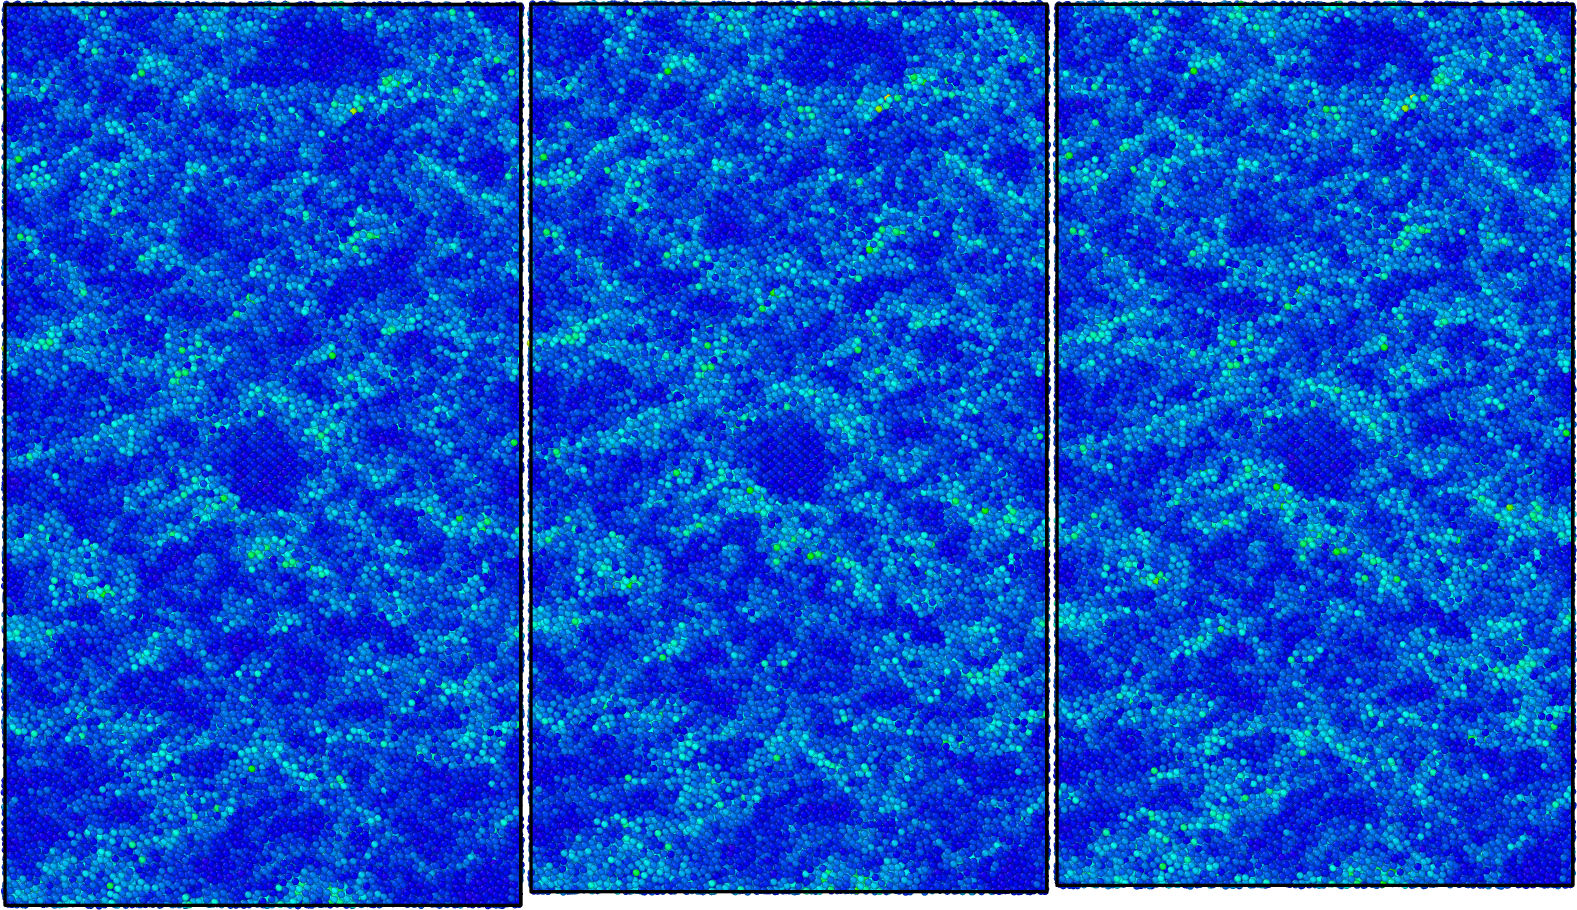
\includegraphics[width=10cm]{../ResumenImagenes/Figures/NanoParticles/Snapshots/B2SphereCompression_200K_Snapshots.png}
\caption{Inclusión de CuZr-B2 bajo compresión a 200K}
\label{C4:fg:snapshot_comp_B2_200K}
\end{figure}

\begin{figure}[htp]
\centering
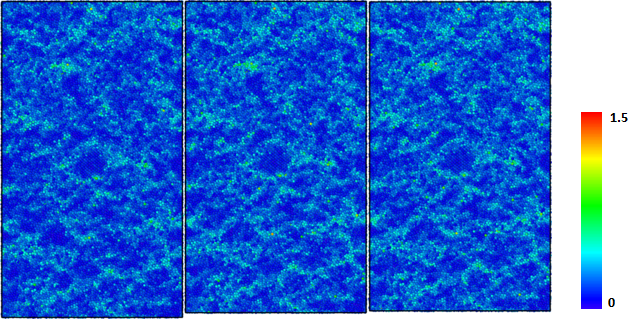
\includegraphics[width=10cm]{../ResumenImagenes/Figures/NanoParticles/Snapshots/B2SphereCompression_300K_Snapshots.png}
\caption{Inclusión de CuZr-B2 bajo compresión a 300K}
\label{C4:fg:snapshot_comp_B2_300K}
\end{figure}

\begin{figure}[htp]
\centering
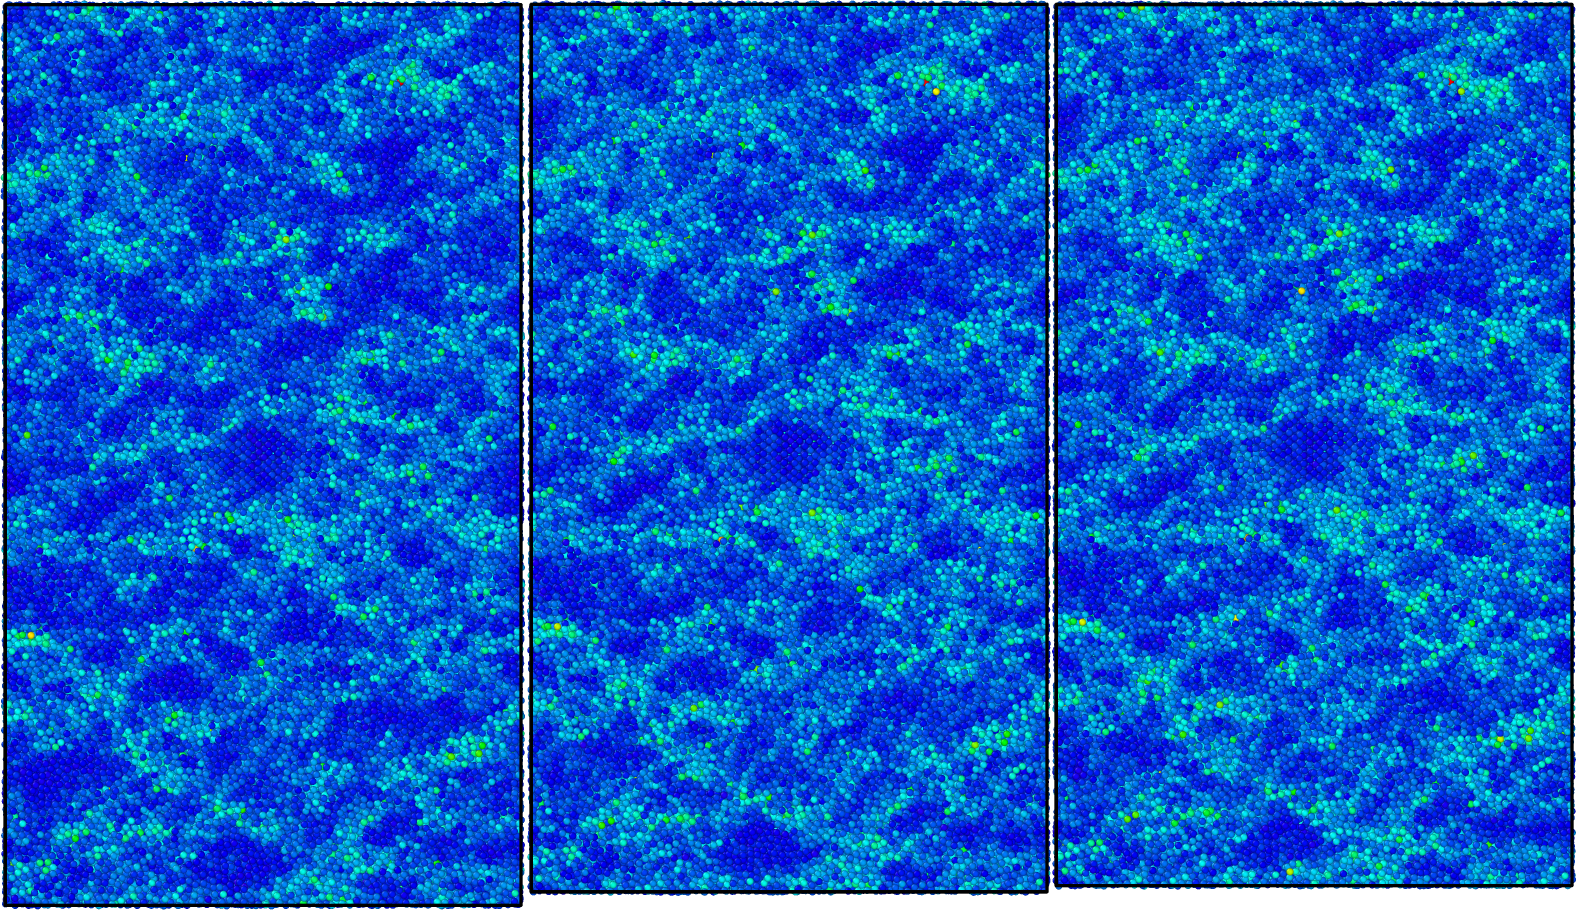
\includegraphics[width=10cm]{../ResumenImagenes/Figures/NanoParticles/Snapshots/B2SphereCompression_400K_Snapshots.png}
\caption{Inclusión de CuZr-B2 bajo compresión a 400K}
\label{C4:fg:snapshot_comp_B2_400K}
\end{figure}

\begin{figure}[htp]
\centering
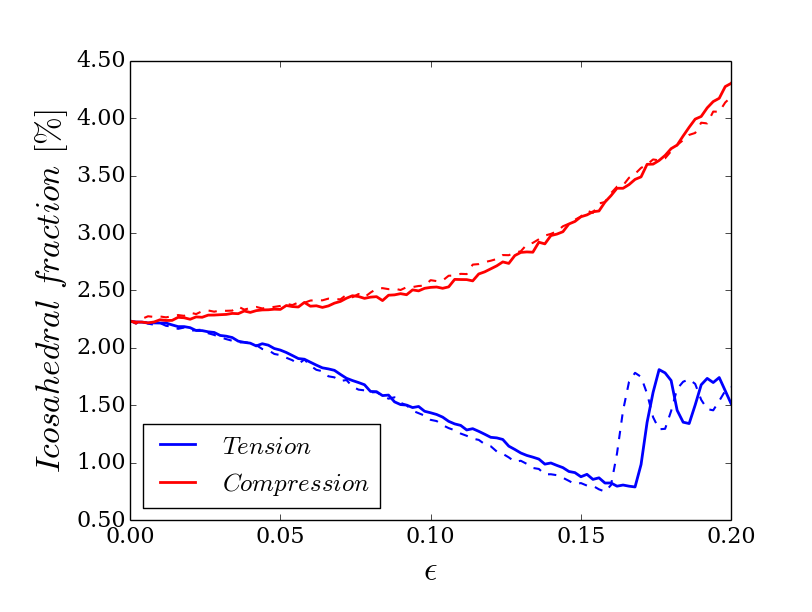
\includegraphics[width=12cm]{Cap_4/FCC_voro_vs_strain_10K_B.png}
\caption[Fracción de icosaedros a 10K]{Fracción de icosaedros bajo tracción y compresión a 10 K. La línea punteada representa la muestra original.}
\label{C4:fg:fcc_voro_10K}
\end{figure}

\section{Resumen y Conclusiones}
\label{S4_4}

Estudiamos un BMG con una nanopartícula cristalina como inclusión. Consideramos un vidrio CuZr, y una nanopartícula de Cu pura con un radio de 2 nm. Ésto implica una fracción en volumen que varía desde 1.15\% a 10 K hasta 1.12\% a 800 K como resultado del aumento del volumen inicial de la muestra con la temperatura. Una situación similar fue explorada recientemente por Albe et al. \cite{albe13}. Aquí, nos centramos en los efectos de la temperatura, e inicialmente estudiamos la estabilidad debajo de los 400 K, indicando que la nanopartícula es bastante estable a esas temperaturas. A temperaturas mayores, la difusividad en sólo algunos ns trae consigo la pérdida de una interfaz nítida entre la nanopartícula y la matriz.

En nuestras simulaciones, se aplicaron condiciones de frontera periódicas en tres dimensiones, y la ausencia de superficies libres deja sólo a la nanopartícula como probable concentrador de esfuerzo para promover la nucleación de STZs, y así desencadenar las bandas de corte, en la interfaz entre la matriz y la nanopartícula. Sin embargo, éste no fue el caso. Las curvas de esfuerzo-deformación son claramente similares al caso sin nanopartícula, a excepción de un retardo en la nucleación de un poro bajo tracción para la muestra con una nanopartícula.

El análisis de Voronoi no muestra diferencias significativas entre las muestras con y sin inclusión de nanopartícula. Un estudio futuro y más detallado es requerido para diferentes modos de carga y temperaturas. Estudios futuros también podrían repetir estos experimentos con inclusiones de CuZr con una estructura cristalina B2, como podemos encontrar en algunas experiencias (\cite{wei14}, \cite{kuo14}).